\chapter{Experimentación}
\label{cap:experimentacion}
En este capitulo desarrollaremos e ilustraremos los diferentes experimentos o pruebas unitarias que se han realizado para la validación del sistema de mapeado dinámico y el sistema de navegación semántica. En primer lugar se realizarán test de mapeado en un entorno doméstico. Con esto comprobaremos que los objetos son eliminados del mapa si desaparecen y como el mapa va cambiando. También haremos pruebas en una estancia de la casa que no aparece en los mapas y comprobaremos como se añade correctamente al mapa. En segundo lugar haremos pruebas de navegación en un entorno doméstico y dinámico y por ultimo expondremos los experimentos llevados a cabo en la RoboCup@Home en el transcurso de la competición.

\section {Mapeado en entorno doméstico}
\label{cap:mapeadodomestico}
En esta primera sección se expondrán los experimentos realizados para validar el proceso por el cual se incluyen o se eliminan los objetos del primer mapa que maneja el servidor de mapas dinámico, el mapa de corto plazo. Estos experimentos se realizarán primero en el simulador Gazebo con el mapa GrannieAnnie, y después en el robot real en el laboratorio.

\subsection {Adición y eliminación de objetos en el mapa de corto plazo en entorno simulado}
\label{sec:add-deleteobjects}

La figura \ref{fig:initserver} fue captada al iniciar el algoritmo. Observamos que la mayor parte del mapa de corto plazo se encuentra en una posición de desconocimiento y que se han ido incluyendo en este las zonas libres, las paredes y la estantería. Los puntos morados y verdes corresponden a la representación de las muestras tomadas por el láser.

\begin{figure}[hbtp]
  \begin{center}
    \subfigure[]{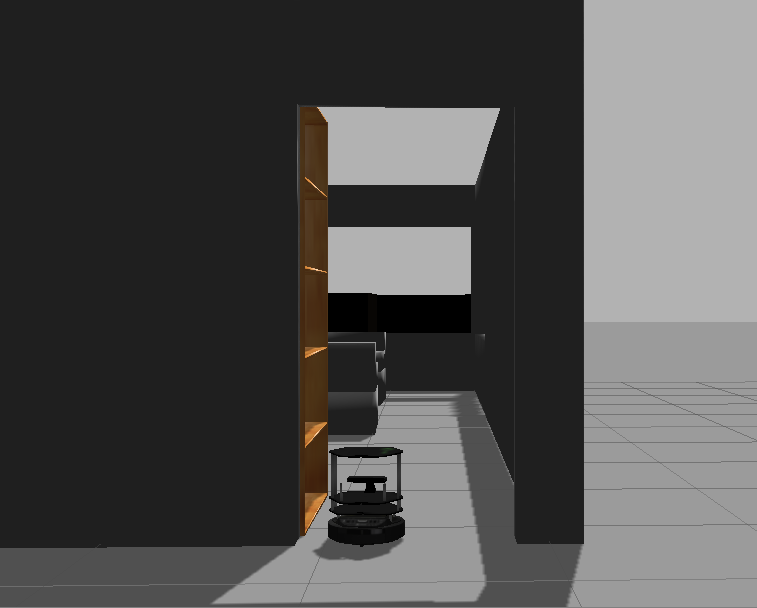
\includegraphics[width=5cm,height=5cm]{img/cap7/incrementmap}}
    \subfigure[]{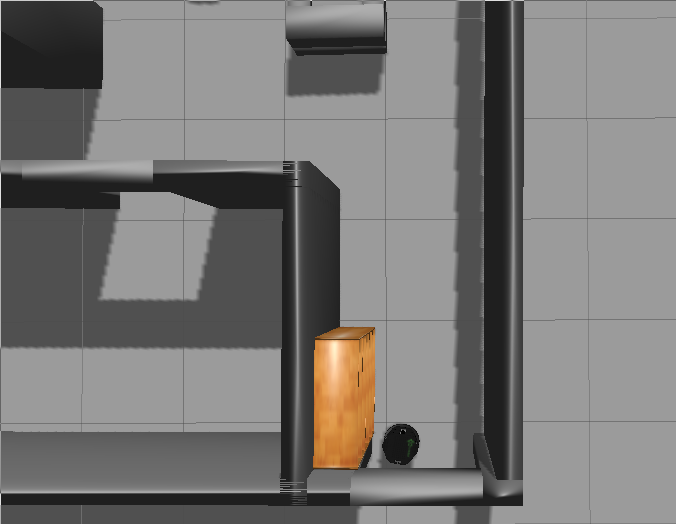
\includegraphics[width=5cm,height=5cm]{img/cap7/incrementmap2}}
    \subfigure[]{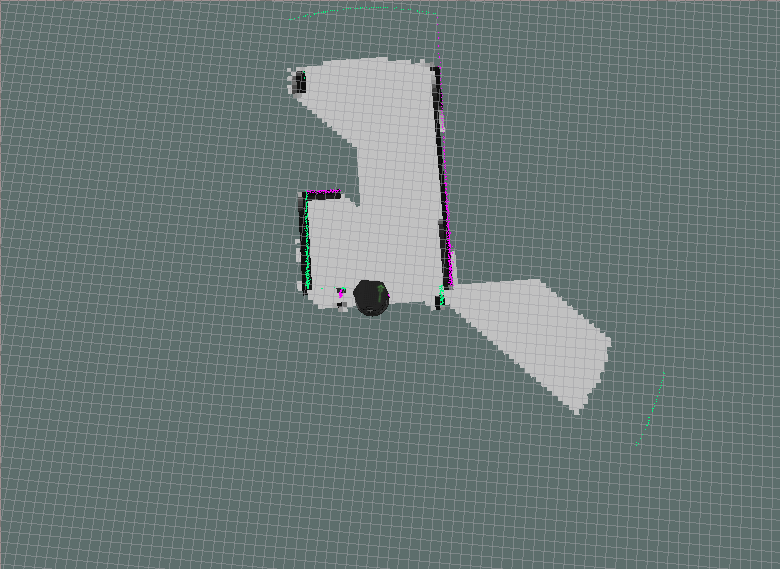
\includegraphics[width=5cm,height=5cm]{img/cap7/incrementmap-rviz}}
  \end{center}
  \caption{Visión del simulador, (a) y (b), y mapa a corto plazo (c).}
  \label{fig:initserver}
\end{figure}

Tras el inicio del algoritmo se añadió un objeto nuevo al escenario. Esto se representa en la figura \ref{fig:includeobject}. Vemos como el objeto ha sido reconocido por el láser, ya que podemos observar su contorno en las marcas de colores verdes y que el algoritmo añade el objeto al mapa y lo sitúa en una posición coherente respecto a la posición que ocupa el objeto en el escenario simulado.

\begin{figure} [hbtp]
  \begin{center}
    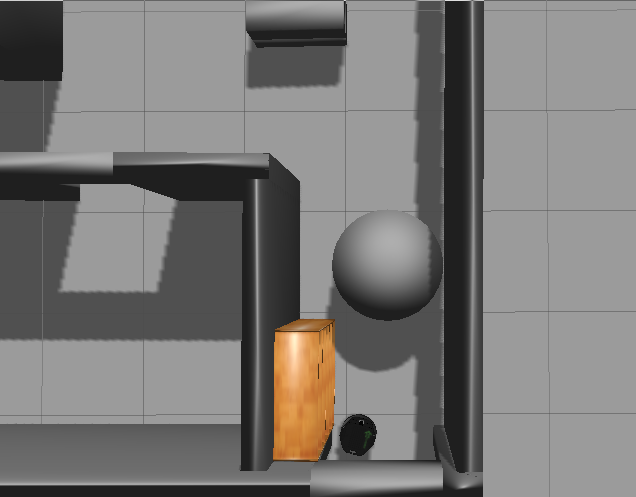
\includegraphics[width=6cm,height=5cm]{img/cap7/incrementmap-object3}
    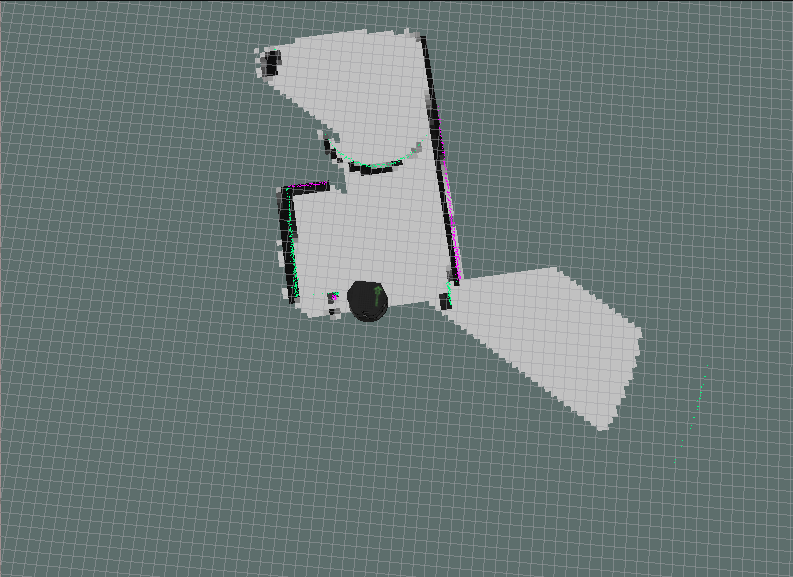
\includegraphics[width=6cm,height=5cm]{img/cap7/incrementmap-object}
  \end{center}
  \caption{Añadimos un objeto al escenario}
  \label{fig:includeobject}
\end{figure}

Una vez que el algoritmo a incluido el objeto en el mapa procedemos a eliminarlo del escenario simulado. Se observa también que las marcas del láser ya no aparecen superpuestas en el mapa. Esto se representa en la figura  \ref{fig:deleteobject}. Vemos como el algoritmo ha comenzado a borrar el objeto, por lo que el valor de las celdas que estaban ocupadas por el objeto ahora es mucho menor.

\begin{figure}[hbtp]
  \begin{center}
    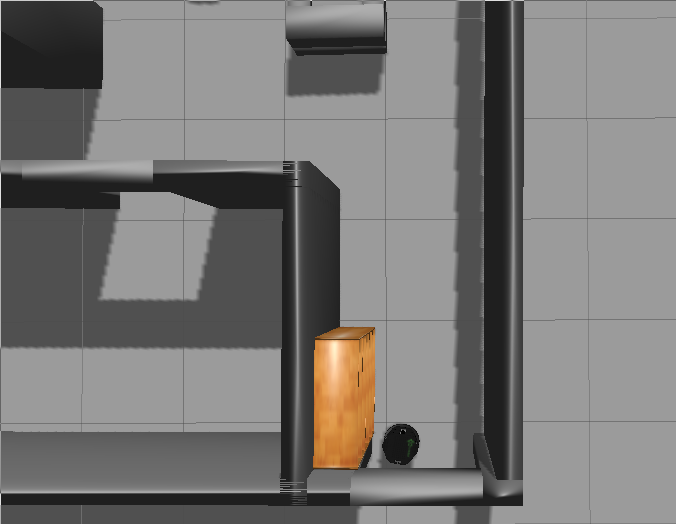
\includegraphics[width=6cm,height=5cm]{img/cap7/incrementmap2}
    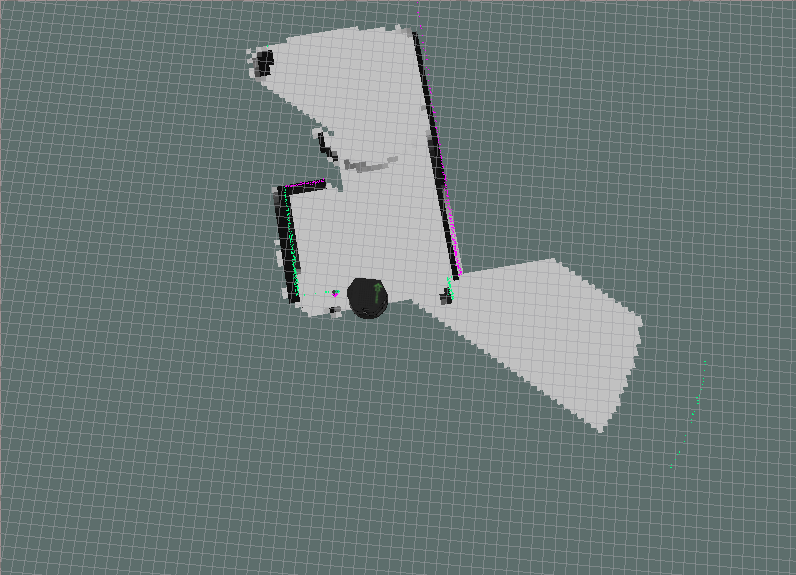
\includegraphics[width=6cm,height=5cm]{img/cap7/incrementmap-object2}
  \end{center}
  \caption{Eliminamos un objeto del escenario}
  \label{fig:deleteobject}
\end{figure}

\subsection {Adición y eliminación de objetos en el mapa de corto plazo en entorno real}
\label{sec:add-deleteobjectsreal}

GRAFICA ADICION: RELACION VALOR VARIABLE / TIEMPO
GRAFICA BORRADO: RELACION VALOR VARIABLE / TIEMPO

\subsection {Adición y eliminación de objetos en el mapa de largo plazo en entorno simulado}
\label{sec:add-deleteobjectslong}
En el siguiente experimento probaremos el añadido y borrado de objetos en el mapa de largo plazo. Para ello realizamos el mismo experimento que en la sección anterior aunque ahora el objeto en el camino del robot es un sofá. Observamos en la figura \ref{fig:addobjectlongmap} como se encuentra el nuevo objeto y al cabo de un tiempo lo añade al mapa de largo plazo. 
\begin{figure}[hbtp]
  \begin{center}
    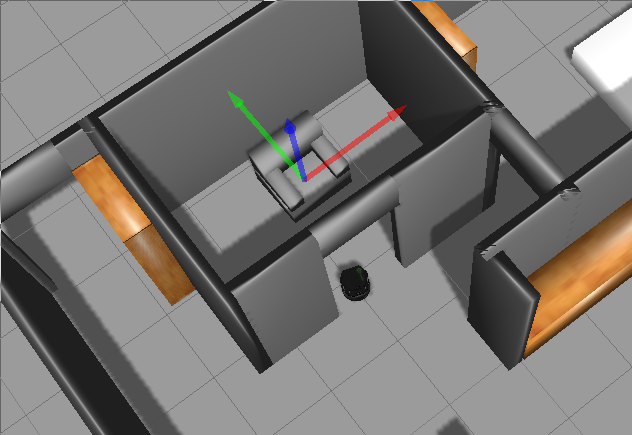
\includegraphics[width=10cm,height=6cm]{img/cap7/addingobject-gazebo}
    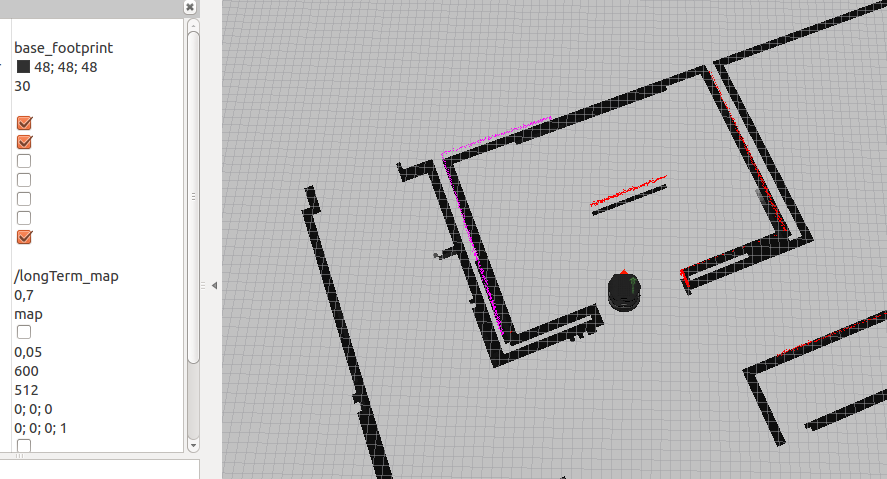
\includegraphics[width=10cm,height=5cm]{img/cap7/addingobject-longmap}
  \end{center}
  \caption{Añadimos un objeto al mapa de largo plazo}
  \label{fig:addobjectlongmap}
\end{figure}
En la figura \ref{fig:deleteobjectlongmap} el objeto ha sido eliminado del entorno simulado y el algoritmo comienza a borrarlo también del mapa de largo plazo. Observamos como ha disminuido el valor de las celdas ocupadas anteriormente por el sofá.

\begin{figure}[hbtp]
  \begin{center}
    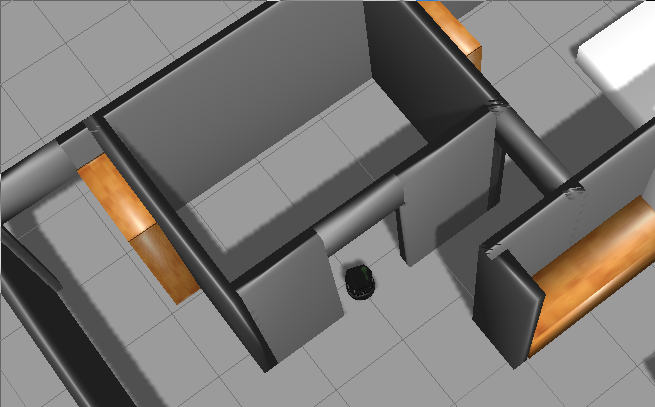
\includegraphics[width=10cm,height=5cm]{img/cap7/deletingobject-gazebo}
    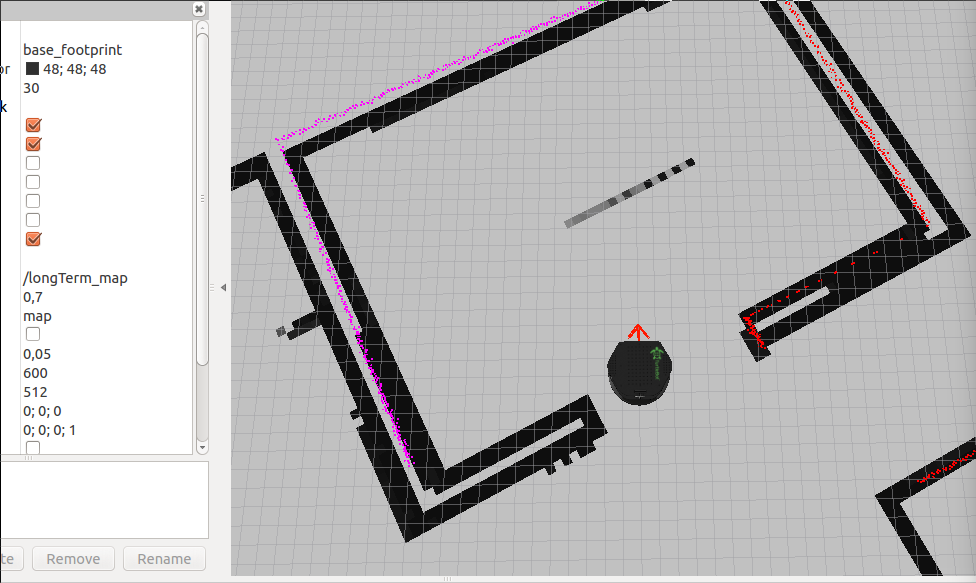
\includegraphics[width=10cm,height=5cm]{img/cap7/deletingobject-longmap}
  \end{center}
  \caption{Borramos un objeto del mapa de largo plazo}
  \label{fig:deleteobjectlongmap}
\end{figure}

GRAFICA BORRADO: RELACION VALOR VARIABLE / TIEMPO

\subsection {Mapeado de zonas desconocidas.}
Para este experimento se ha extendido ligeramente el mapa simulado, de tal forma que se han añadido unos pasillos nuevos a la derecha del escenario, como vemos en la figura \ref{fig:grannieAnne-ext}. Esta zona no vamos a incluirla previamente en el mapa estático ni en el mapa de largo plazo y queremos comprobar si el sistema es capaz de añadir una zona nueva al mapa y localizarse correctamente. El mapa estático usado es el mismo que el mostrado en la figura \ref{fig:mapaestatico}.
\begin{figure}[H]
  \begin{center}
    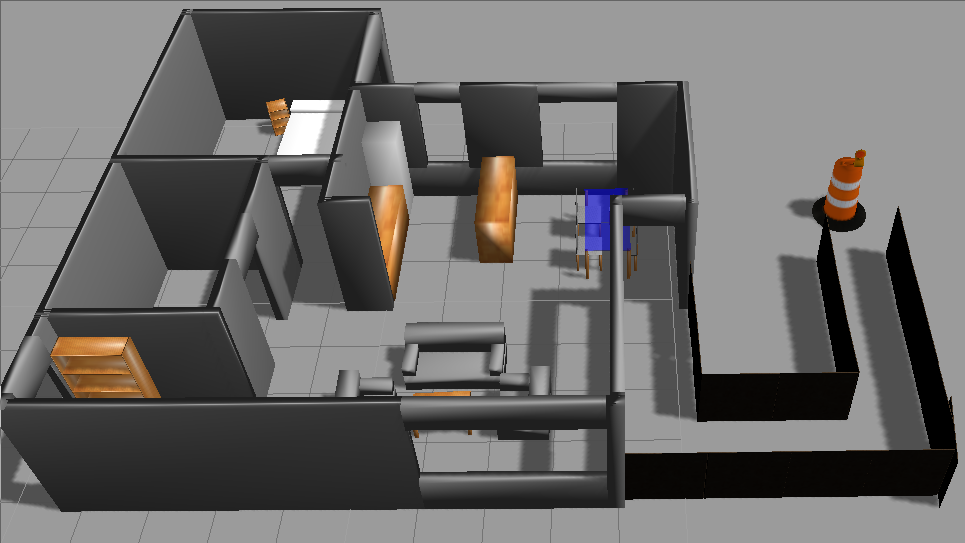
\includegraphics[width=12cm,height=7cm]{img/cap7/grannieAnne-ext}
  \end{center}
  \caption{Escenario extendido}
  \label{fig:grannieAnne-ext}
\end{figure}

\begin{figure}[hbtp]
  \begin{center}
    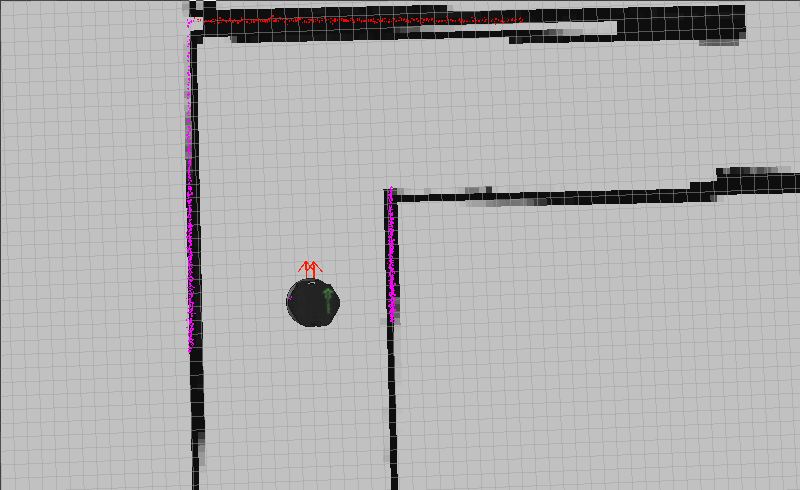
\includegraphics[width=10cm,height=6cm]{img/cap7/localization-ext}
  \end{center}
  \caption{Detalle de la localización}
  \label{fig:localization-ext}
\end{figure}

\begin{figure}[hbtp]
  \begin{center}
    \subfigure[Mapa total]{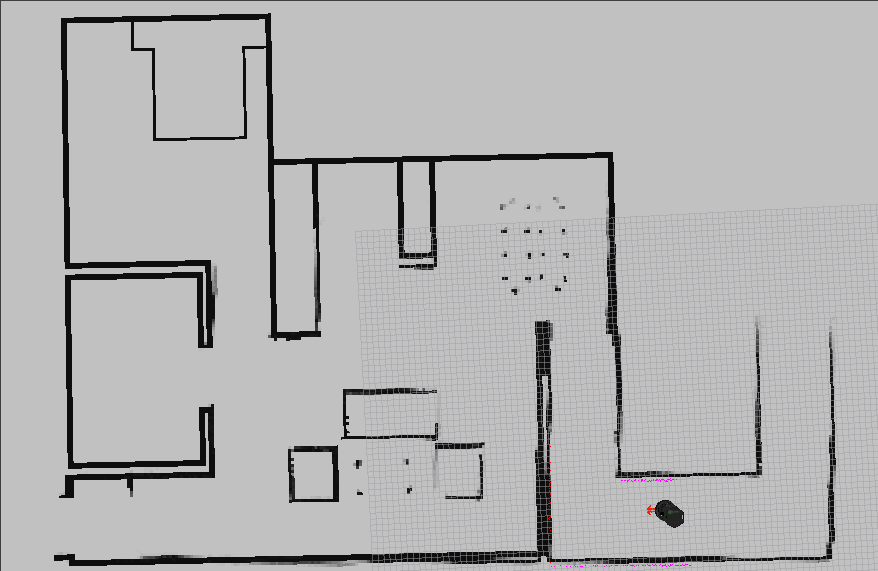
\includegraphics[width=12cm,height=7cm]{img/cap7/map-ext}}
    \subfigure[Mapa de largo plazo]{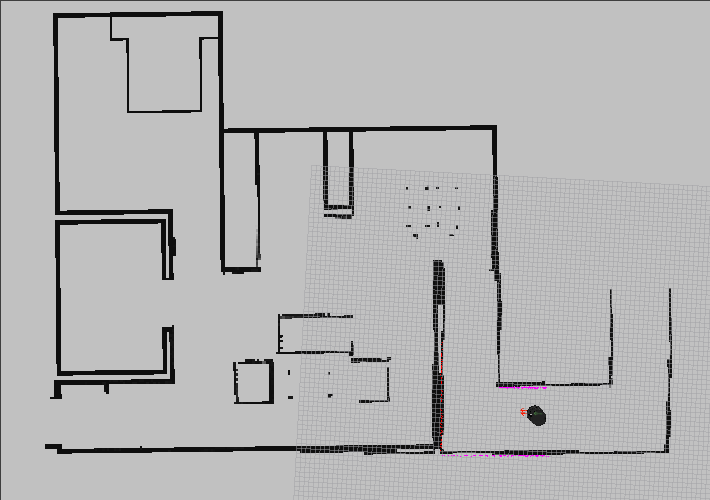
\includegraphics[width=12cm,height=7cm]{img/cap7/longmap-ext}}
    \subfigure[Mapa de corto plazo]{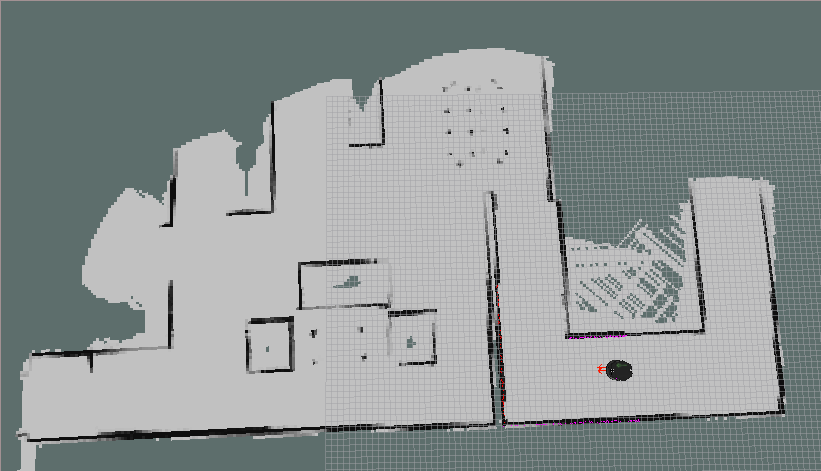
\includegraphics[width=12cm,height=7cm]{img/cap7/shortmap-ext}}
  \end{center}
  \caption{Mapas del escenario extendido}
  \label{fig:maps-ext}
\end{figure}

  Vemos como después de recorrer la parte desconocida del mapa se ha añadido al mapa de largo plazo y también al mapa total, figura \ref{fig:maps-ext}. Observamos en las flechas rojas bajo el robot que la incertidumbre en la posición del robot es mínima, figura \ref{fig:localization-ext}. Comprobamos con este experimento la potencia de esta característica de nuestro sistema, somos capaces de añadir zonas completas al mapa sin necesidad de reiniciar el algoritmo ni de modificar el mapa estático, y seguir completamente localizados.

\subsection {Adición y eliminación de objetos en el mapa de largo plazo en entorno real}
\label{sec:add-deleteobjectslongreal}

\section {Navegación con obstáculos dinámicos}
\label{cap:navegacionconobstaculos}

\section {Experimentación en la Robocup}
\label{cap:experimentacionrobocup}










